\documentclass{beamer}
\usetheme{Rochester}
\usecolortheme{default}

\usepackage[utf8]{inputenc}
\usepackage{german}

\title{App zur Inventarisierung von Unternehmenswerten}
\author{Gruppe ak18b}
\date{28. März 2019}

\begin{document}	
	\begin{frame}
	\begin{figure}
		
\includegraphics[scale=0.25]{Logo.png}
	\end{figure}
	\begin{center}
		\vskip -1em
		\tiny Wintersemester 2018/19\\
		\tiny Softwaretechnikpraktikum
	\end{center}
	\vskip -2em
	\titlepage
\end{frame}

%\frame{\frametitle{Inhaltsverzeichnis}
%	\tableofcontents}

\section{Demonstration}
\frame{
	\frametitle{Demostration}
	\centering{\textcolor{blue}{\url{http://pcai042.informatik.uni-leipzig.de:1590}}}
}

\section{Technische Umsetzung des UserInterfaces}
\frame{\frametitle{Technische Umsetzung des UserInterfaces (UI)}
\centering{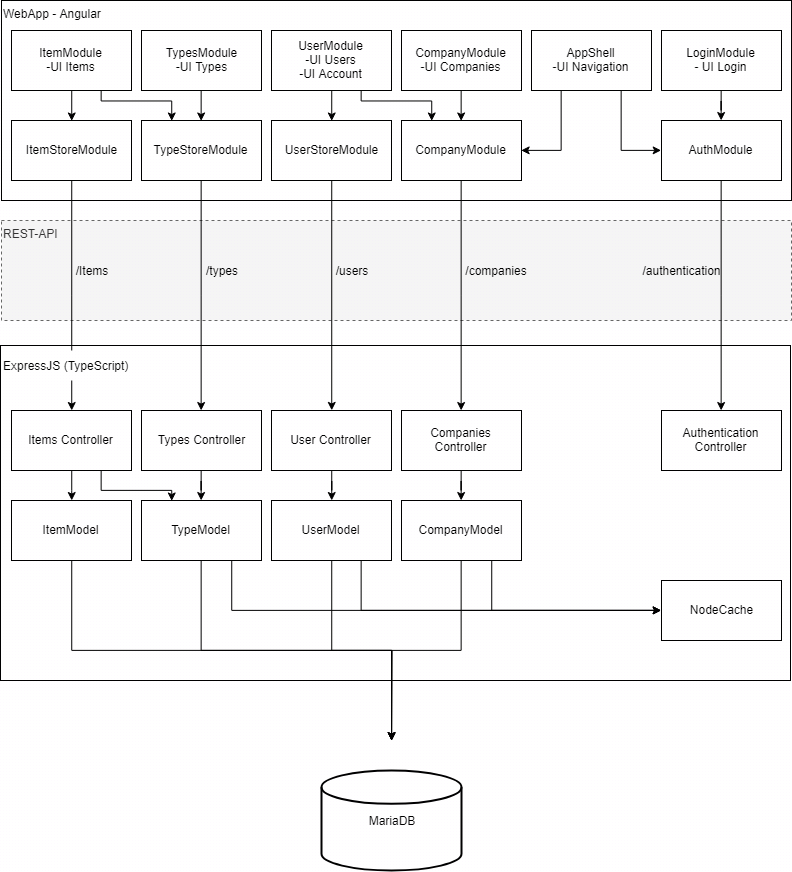
\includegraphics[scale=0.25]{architecture.png}}
}

\section{Datenhandling in der UI}
\begin{frame}{Datenhandling in der UI}
Jede kontext-getrennte Ressource hat einen eigenen sogenannten \glqq Store\grqq\\
Ein Store bietet 6 Methoden: 
\texttt{
\begin{itemize}
	\item load()
	\item byId(id)
	\item create(enitity)
	\item update(enitity)
	\item delete(id)
	\item store
\end{itemize}}
\end{frame}

\section{Lessons learned}
\begin{frame}{Lessons learned}
\begin{itemize}
	\item Einstieg in Angular ziemlich schwer
	\item TypeScript nicht so fehlertollerant wie JavaScript
	\item Besser recherchieren vor und während des Projekts
	\item Reviewgespräche besser vorbereiten
	\item Zeit besser einteilen
\end{itemize}
\end{frame}


\end{document}
